%%%
% Plantilla de Memoria
% Modificación de una plantilla de Latex de Nicolas Diaz para adaptarla 
% al castellano y a las necesidades de escribir informática y matemáticas.
%
% Editada por: Mario Román
%
% License:
% CC BY-NC-SA 3.0 (http://creativecommons.org/licenses/by-nc-sa/3.0/)
%%%

%%%%%%%%%%%%%%%%%%%%%%%%%%%%%%%%%%%%%%%%%
% Thin Sectioned Essay
% LaTeX Template
% Version 1.0 (3/8/13)
%
% This template has been downloaded from:
% http://www.LaTeXTemplates.com
%
% Original Author:
% Nicolas Diaz (nsdiaz@uc.cl) with extensive modifications by:
% Vel (vel@latextemplates.com)
%
% License:
% CC BY-NC-SA 3.0 (http://creativecommons.org/licenses/by-nc-sa/3.0/)
%
%%%%%%%%%%%%%%%%%%%%%%%%%%%%%%%%%%%%%%%%%

%----------------------------------------------------------------------------------------
%	PAQUETES Y CONFIGURACIÓN DEL DOCUMENTO
%----------------------------------------------------------------------------------------
%%% Configuración del papel.
% microtype: Tipografía.
% mathpazo: Usa la fuente Palatino.
\documentclass[a4paper, 11pt]{article}
\usepackage[protrusion=true,expansion=true]{microtype}
\usepackage{mathpazo}

\usepackage{fancyvrb}

% redefine \VerbatimInput
\RecustomVerbatimCommand{\VerbatimInput}{VerbatimInput}%
{fontsize=\footnotesize,
	%
	frame=lines,  % top and bottom rule only
	framesep=2em, % separation between frame and text
	rulecolor=\color{Gray},
	%
	label=\fbox{\color{Black}data.txt},
	labelposition=topline,
	%
	commandchars=\|\(\), % escape character and argument delimiters for
	% commands within the verbatim
	commentchar=*        % comment character
}



% Indentación de párrafos para Palatino
\setlength{\parindent}{0pt}
  \parskip=8pt
\linespread{1.05} % Change line spacing here, Palatino benefits from a slight increase by default




%%% Castellano.
% noquoting: Permite uso de comillas no españolas.
% lcroman: Permite la enumeración con numerales romanos en minúscula.
% fontenc: Usa la fuente completa para que pueda copiarse correctamente del pdf.
\usepackage[spanish,es-noquoting,es-lcroman]{babel}
\usepackage[utf8]{inputenc}
\usepackage[T1]{fontenc}
\selectlanguage{spanish}




%%% Gráficos
\usepackage{graphicx} % Required for including pictures
\usepackage{wrapfig} % Allows in-line images
\usepackage[usenames,dvipsnames]{color} % Coloring code

%%% Matemáticas
\usepackage{amsmath}


%%% Bibliografía
\makeatletter
\renewcommand\@biblabel[1]{\textbf{#1.}} % Change the square brackets for each bibliography item from '[1]' to '1.'
\renewcommand{\@listI}{\itemsep=0pt} % Reduce the space between items in the itemize and enumerate environments and the bibliography

%% ENLACES 
\usepackage{hyperref}
\hypersetup{
	colorlinks   = true,    % Colours links instead of ugly boxes
	urlcolor     = MidnightBlue,    % Colour for external hyperlinks
	linkcolor    = MidnightBlue, %BurntOrange,    % Colour of internal links
	citecolor    = MidnightBlue      % Colour of citations
}

%% codigo

%%% CÓDIGO
 \usepackage{listings}
\usepackage{courier}
\lstset{
	basicstyle=\footnotesize\ttfamily, % Standardschrift
	numbers=left,               % Ort der Zeilennummern
	numberstyle=\tiny,          % Stil der Zeilennummern
	stepnumber=1,               % Abstand zwischen den Zeilennummern
	numbersep=5pt,              % Abstand der Nummern zum Text
	tabsize=2,                  % Groesse von Tabs
	extendedchars=true,         %
	breaklines=true,            % Zeilen werden Umgebrochen
	keywordstyle=\color{red},
	frame=b,         
	%        keywordstyle=[1]\textbf,    % Stil der Keywords
	%        keywordstyle=[2]\textbf,    %
	%        keywordstyle=[3]\textbf,    %
	%        keywordstyle=[4]\textbf,   \sqrt{\sqrt{}} %
	stringstyle=\color{white}\ttfamily, % Farbe der String
	showspaces=false,           % Leerzeichen anzeigen ?
	showtabs=false,             % Tabs anzeigen ?
	xleftmargin=17pt,
	framexleftmargin=17pt,
	framexrightmargin=5pt,
	framexbottommargin=4pt,
	%backgroundcolor=\color{lightgray}
	showstringspaces=false      % Leerzeichen in Strings anzeigen ?        
	literate=
	{á}{{\'a}}1 {é}{{\'e}}1 {í}{{\'i}}1 {ó}{{\'o}}1 {ú}{{\'u}}1
	{Á}{{\'A}}1 {É}{{\'E}}1 {Í}{{\'I}}1 {Ó}{{\'O}}1 {Ú}{{\'U}}1
	{à}{{\`a}}1 {è}{{\`e}}1 {ì}{{\`i}}1 {ò}{{\`o}}1 {ù}{{\`u}}1
	{À}{{\`A}}1 {È}{{\'E}}1 {Ì}{{\`I}}1 {Ò}{{\`O}}1 {Ù}{{\`U}}1
	{ä}{{\"a}}1 {ë}{{\"e}}1 {ï}{{\"i}}1 {ö}{{\"o}}1 {ü}{{\"u}}1
	{Ä}{{\"A}}1 {Ë}{{\"E}}1 {Ï}{{\"I}}1 {Ö}{{\"O}}1 {Ü}{{\"U}}1
	{â}{{\^a}}1 {ê}{{\^e}}1 {î}{{\^i}}1 {ô}{{\^o}}1 {û}{{\^u}}1
	{Â}{{\^A}}1 {Ê}{{\^E}}1 {Î}{{\^I}}1 {Ô}{{\^O}}1 {Û}{{\^U}}1
	{œ}{{\oe}}1 {Œ}{{\OE}}1 {æ}{{\ae}}1 {Æ}{{\AE}}1 {ß}{{\ss}}1
	{ű}{{\H{u}}}1 {Ű}{{\H{U}}}1 {ő}{{\H{o}}}1 {Ő}{{\H{O}}}1
	{ç}{{\c c}}1 {Ç}{{\c C}}1 {ø}{{\o}}1 {å}{{\r a}}1 {Å}{{\r A}}1
	{€}{{\euro}}1 {£}{{\pounds}}1 {«}{{\guillemotleft}}1
	{»}{{\guillemotright}}1 {ñ}{{\~n}}1 {Ñ}{{\~N}}1 {¿}{{?`}}1   
}


\lstloadlanguages{% Check Dokumentation for further languages ...
%[Visual]Basic
%Pascal
%C
C++
%%XML
%%HTML
%Java
}
%\DeclareCaptionFont{blue}{\color{blue}} 

%\captionsetup[lstlisting]{singlelinecheck=false, labelfont={blue}, textfont={blue}}
\usepackage{caption}
\DeclareCaptionFont{white}{\color{white}}
\DeclareCaptionFormat{listing}{\colorbox[cmyk]{0.43, 0.35, 0.35,0.01}{\parbox{\textwidth}{\hspace{15pt}#1#2#3}}}
\captionsetup[lstlisting]{format=listing,labelfont=white,textfont=white, singlelinecheck=false, margin=0pt, font={bf,footnotesize}
}

%% cosas 

\usepackage[margin=1in]{geometry}

\usepackage{times}


%% colorear titulos
\usepackage{titlesec}
\titleformat{\section}
{\color{MidnightBlue}\normalfont\Large\bfseries}
{\color{Black}\thesection}{1em}{}


%% CREAR DIAGRAMAS 

\usepackage{tikz}

%% rodear figura de texto
\usepackage{graphicx,wrapfig,lipsum}
 %% comentarios multilinea
\usepackage{verbatim}

\definecolor{darkGray}{gray}{0.05}

%----------------------------------------------------------------------------------------
%	DOCUMENTO
%----------------------------------------------------------------------------------------

\begin{document}
	
	
	\begin{titlepage}
		\begin{center}
			\vspace*{0.2cm}
			
			{\Huge \textbf{\textcolor{red}{ALGORÍTMICA}}}
			
						{\textcolor[rgb]{0.13,0.09,0.08}	{\Huge\underline{PRÁCTICA 2: DIVIDE Y VENCERÁS}}}
			
				\vspace{0.2cm}
				
				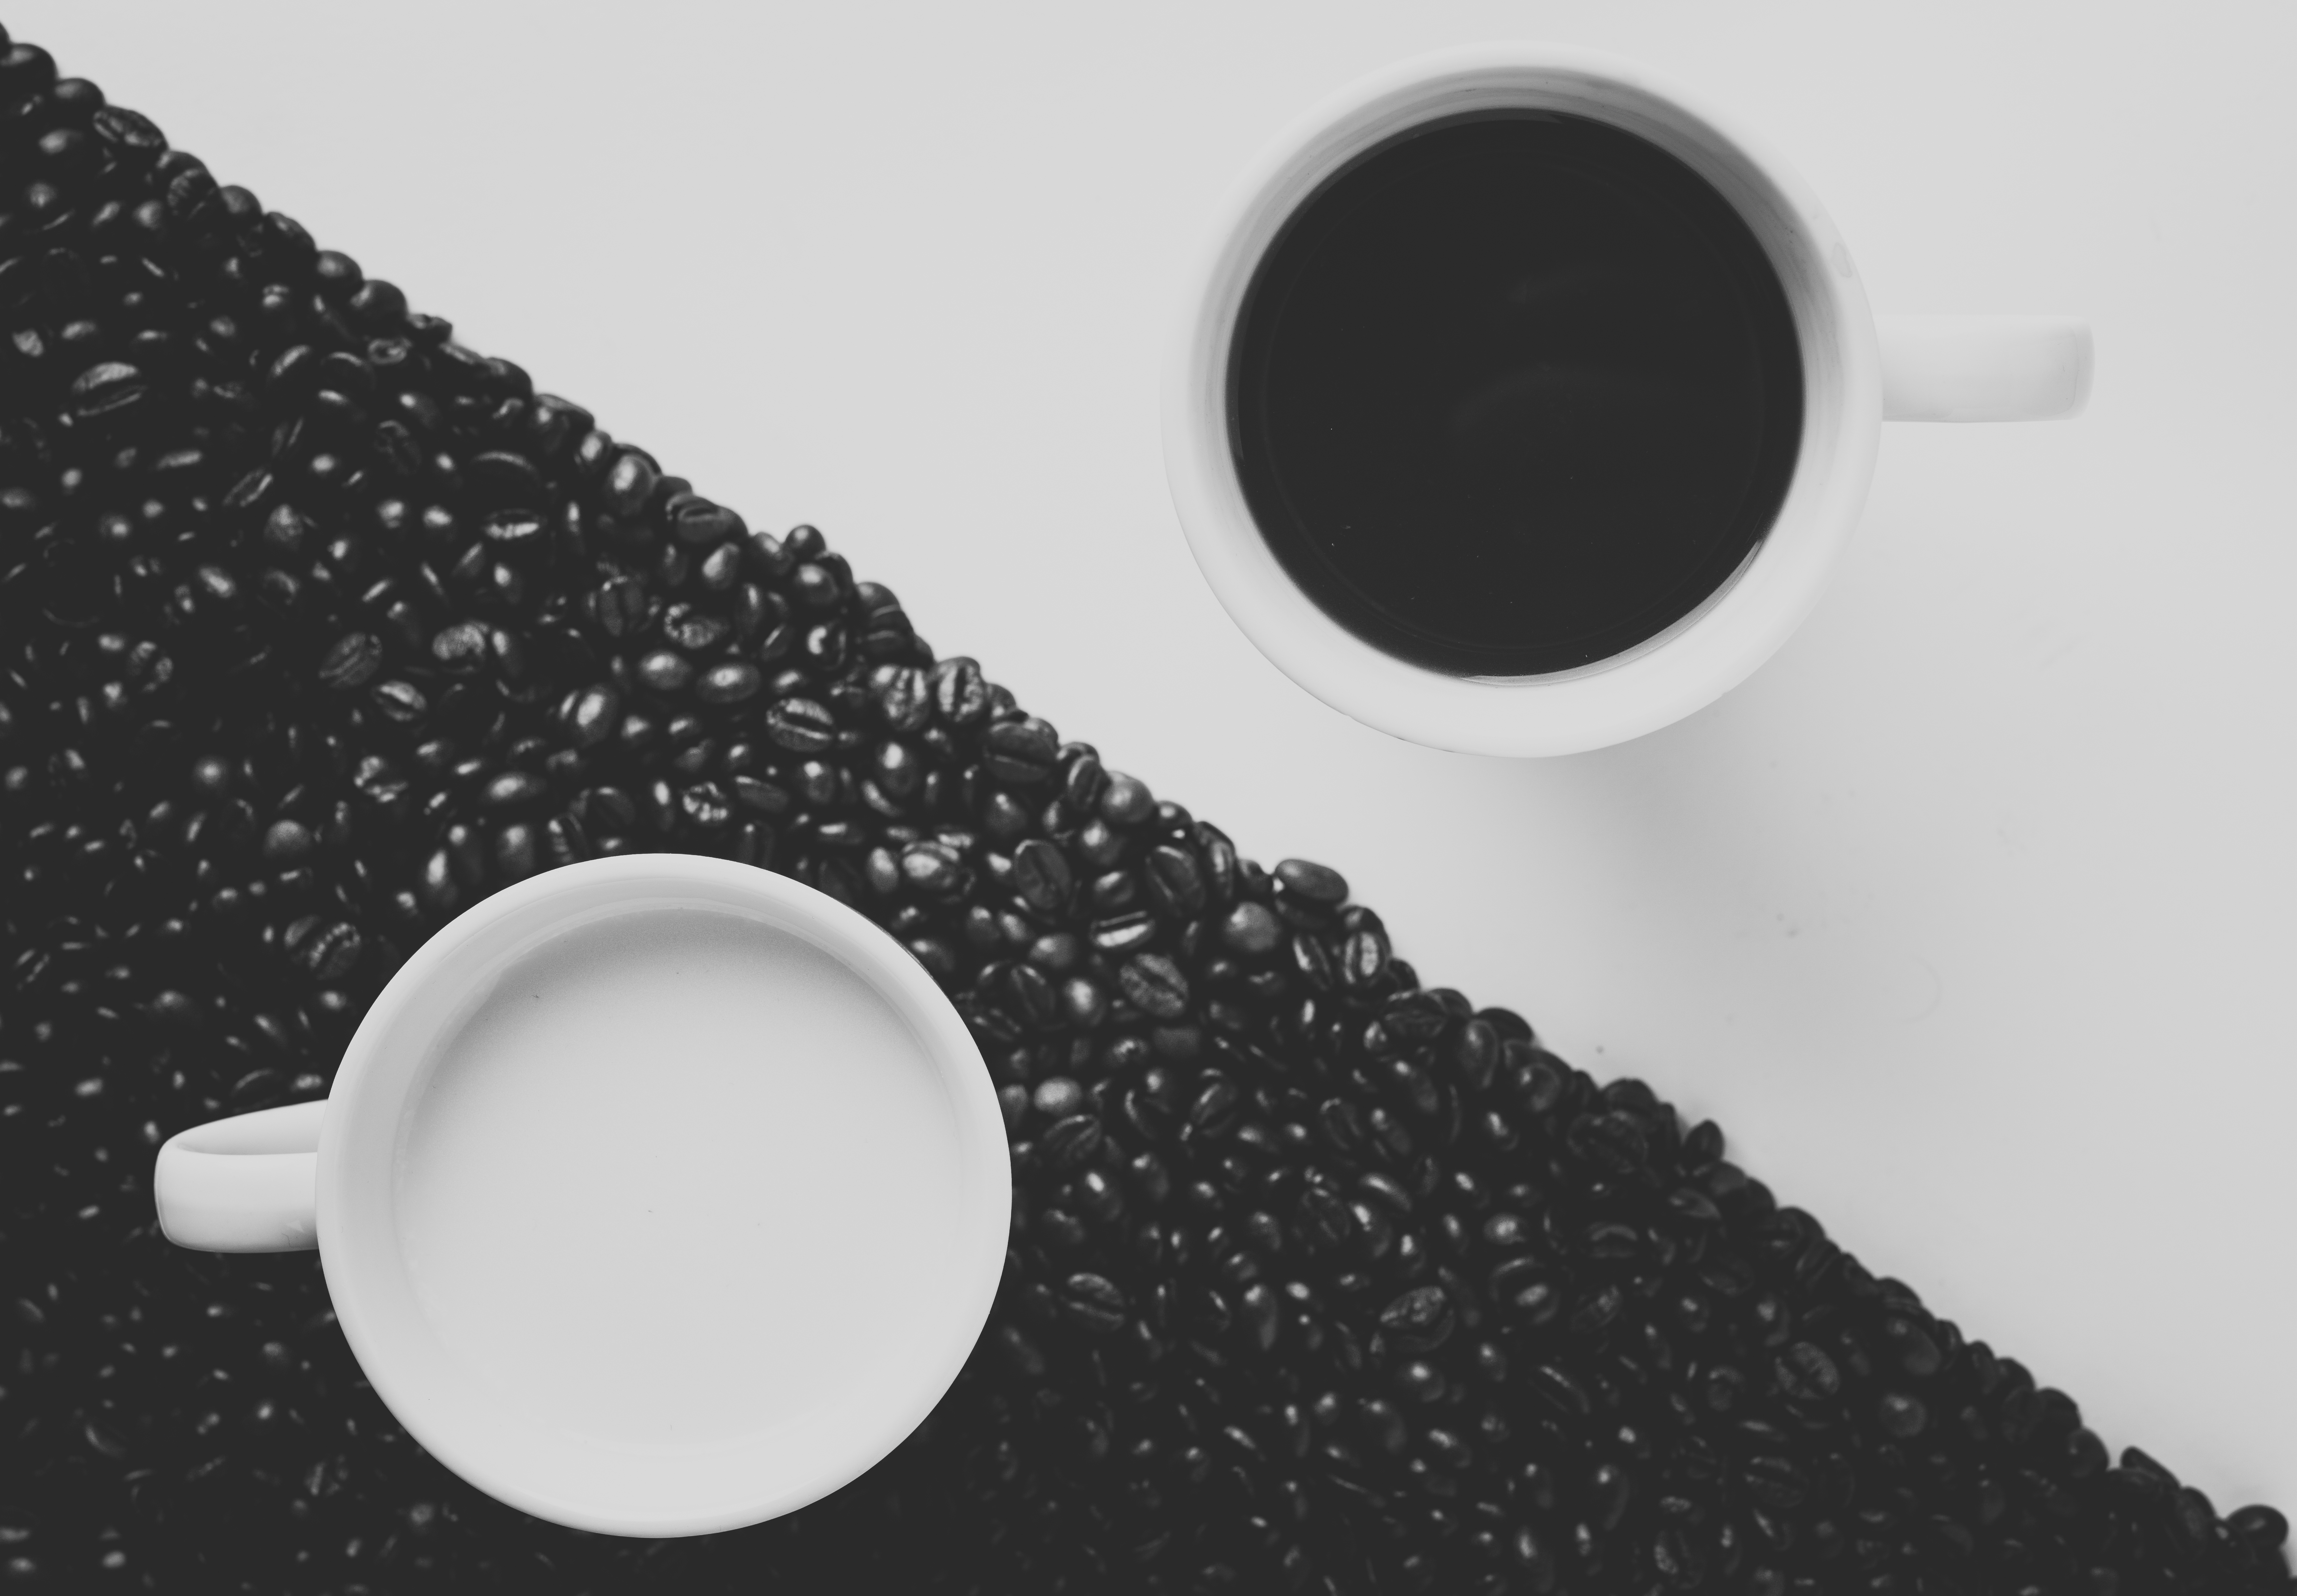
\includegraphics[width=\textwidth]{cover.jpg}
				\vspace{0.2cm}
				

		
			\vspace{1cm}
			
			\textbf{AUTORES: \\
					Pablo Moreno Megías, Diego Lerena García, Manuel Vallejo Felipe, Ángel Díaz de la Torre, Francisco Navarro Morales, Marcel Kemp Muñoz y David Redondo Correa
		    		 }
	    		 \vspace{1cm}
	   
			
			\vfill
			Algorítmica [PRACTICAS]\\
			Segundo curso del Grado de Ingeniería Informática.\\
			Universidad de Granada.\\
			curso 2016-2017.
		\end{center}
	\end{titlepage}


%\maketitle % Print the title section

%% Resumen (Descomentar para usarlo)
\renewcommand{\abstractname}{Resumen} % Uncomment to change the name of the abstract to something else
%\begin{abstract}
% Resumen aquí
%\end{abstract}

%% Palabras clave
%\hspace*{3,6mm}\textit{Keywords:} lorem , ipsum , dolor , sit amet , lectus % Keywords
%\vspace{30pt} % Some vertical space between the abstract and first section

\color{darkGray}
%% Índice
{\parskip=2pt
  \tableofcontents
}
\pagebreak
\section{Problema}

	Dos productos i y j están invertidos en las preferencias de A y B si el usuario
	A prefiere el producto i antes que el j mientras que el usuario B prefiere el
	producto j antes que el i.
	Esto es, cuantas menos inversiones existan entre dos rankings, más similares
	serán las preferencias de los usuarios representados por esos rankings.
	Por ello, el objetivo del problema sería realizar un algoritmo que compruebe el
	número de inversiones que existen entre un vector ordenado, y otro desordenado, sabiendo
	que sus datos van desde 0 hasta n-1 sin que ninguno se repita.
	
\section{Algoritmo Obvio. Fuerza Bruta.}
\subsection{Algoritmo}
	El algoritmo de fuerza bruta comienza comparando la primera posición del vector que nos han dado con todas las demás posiciones del vector, comprobando si el número elegido (primera posición) es mayor que el número con el que se ha comparado. Si se cumpliese esta condición incrementaríamos una variable auxiliar para saber que está mal posicionado. Esta comparación hay que realizarla $n$ veces con todos los números que se encuentren dentro del vector (primer bucle), y además el número elegido debe de compararse con todos los demás números que aún no se hayan comprobado (segundo bucle). El problema de este algoritmo es que tiene una eficiencia muy mala, ya que daría $O(n^2)$, por culpa de los dos bucles anteriormente explicados.
	\lstinputlisting[language=C++,label=Algoritmo de fuerza bruta,caption=Algoritmo de fuerza bruta]{fuerza_bruta.cpp}
\pagebreak
\subsection{Eficiencia teórica.}
Tenemos dos bucles anidados, uno va desde 0 hasta el número de elementos y el otro (interior) va desde el índice del exterior más uno hasta el final, luego tenemos:

$$\sum_{i=0}^{n}\sum_{i+1}^{n}1$$

donde $\sum_{i+1}^{n}1=n-i$ y, al final tenemos, por tanto, $\sum_{i=0}^{n}\sum_{i+1}^{n}1 = \sum_{i=0}^{n}n-i$
Luego tenemos:
$$\sum_{i=0}^{n}n - \sum_{i=0}^{n}i  = n(n+1)-\frac{(n+1)n}{2}= \frac{(n+1)n}{2}=\frac{n^2+n}{2}$$

Luego la eficiencia teórica del algoritmo de fuerza bruta es $O(n^2)$.
\subsection{Eficiencia empírica.}
\begin{figure}[!hbp]
	\includegraphics[width=0.8\textwidth]{algoritmoMalo.png}
	\caption{Algoritmo de fuerza bruta eficiencia empírica	\label{Algoritmo fuerza bruta empírico}}
\end{figure}
\pagebreak
\subsection{Eficiencia híbrida.}
\begin{figure}[!hbp]
	\includegraphics[width=0.8\textwidth]{algoritmoMaloAjuste.png}
	\caption{Algoritmo de fuerza bruta eficiencia híbrida	\label{Algoritmo fuerza bruta hibrido}}
\end{figure}

\begin{figure}[!htp]
	\includegraphics[width=0.8\textwidth]{maloajuste}
	\caption{Ajuste con $n^2$ del algoritmo fuerza bruta\label{AJustemal}}
\end{figure}
\pagebreak
\section{Algoritmo Divide y Vencerás.}
\subsection{Algoritmo}
	\lstinputlisting[language=C++,label=Algoritmo `Divide y vencerás",caption=Algoritmo `Divide y vencerás"]{algoritmoBueno.cpp}
	Nuestra solución consiste en atacar el problema con un esquema de divide y vencerás clásico, basado en dos llamadas recursivas de tamaño $n/2$ y una función para combinar ambas soluciones. La mecánica es: dividimos el problema en dos partes, y cada parte a su vez en dos partes hasta que tengamos problemas de tamaño uno (que tendrán cero inversiones) o de tamaño dos (que tendrán cero o una inversión, dependiendo de si el número mayor está a la izquierda o no). En el caso de tamaño dos, si existe inversión, además de contar dicha inversión, invertimos los dos números para ordenar el vector. 
	Cuando la recursividad `se rompe', nos vemos en la necesidad de, no solo sumar las inversiones en cada mitad en la que dividimos el problema, sino también de contabilizar las inversiones que hay entre los números de una mitad y los de la otra.
	Para ello, tenemos en cuenta que los números de la mitad de la derecha solo podrán tener inversiones con los de la izquierda si los de la izquierda son \textbf{mayores}; y, dado que además nos interesa ir ordenando el vector conforme contamos inversiones, realizamos lo siguiente:
	Como ambas mitades están ordenadas, podemos combinarlas en un vector ordenado en tiempo $O(n)$ simplemente manteniendo un índice para cada parte (empezando en el mínimo de cada una) e ir comparando ambos índices. El de menor valor se introduce en un nuevo vector y se aumenta en uno el valor del índice. Cuando uno de los dos vectores se termine, se introducirán en el vector los elementos restantes del otro hasta que este también termine. Ahora bien, para contar las inversiones tenemos que tener en cuenta el detalle de que \textbf{los vectores están ordenados}. Así, si el elemento del vector de la derecha es menor que un elemento del de la izquierda (que será menor que todos los elementos restantes de este vector, a su derecha); también es menor que todos los elementos que restan de la parte izquierda. Como hemos dicho, tenemos una inversión por cada número de la parte izquierda que sea menor que algún número de la parte de la derecha, así pues, contabilizamos tantas inversiones como números haya a la derecha del índice de la parte izquierda siempre que el valor del vector en dicho índice sea mayor que en el índice de la parte derecha. Así, al mismo tiempo ordenamos el vector (para facilitar cambios posteriores) y contamos las inversiones.

\subsection{Eficiencia teórica.}
El algoritmo de basa en dos llamadas recursivas de tamaño $n/2$ y la combinación de los dos subvectores ordenados obtenidos de ello en $O(n)$.
La condición de parada es si el tamaño es 0, 1 o 2, y en tal caso tarda $O(1)$.
Luego tenemos:

$t(n)=1 para n<3$
$t(n)=2t(n/2)+n$

Si realizamos el cambio $n=b^k\rightarrow k=log_b n$ nos queda: 

$$t(2^k) = 2t(2^{k-1} + 2^k) \rightarrow t(2^k) - 2t(2^{k-1} = 2^k \rightarrow x-2 = 2^k$$

Tenemos una ecuación lineal no homogénea. El polinomio característico de la parte homogénea es x-2, y de la parte no homogénea x-2, también. Luego tenemos una raíz única de multiplicidad 2: $pc=(x-2)^2$ luego la solución general sería:

$$ t(2^k)=c_1 2^k + c_2 k 2^k \rightarrow t(n) = c_1 2^{log_2 n} + c_2 log_2 n \times 2^{log_b n} = c_1 n + c2 log_2 n \times n$$

Como no tiene sentido que $c_1$ y $c_2$ sean negativos, concluimos que la eficiencia del algoritmo es $$O(n \times log_2 n)$$

\subsection{Eficiencia empírica.}
\begin{figure}[!hbp]
	\includegraphics[width=0.8\textwidth]{algBueno.png}
	\caption{Algoritmo divide y vencerás sin ajuste	\label{Algoritmo divide y vencerás análisis empírico}}
\end{figure}
Al medir los tiempos de forma empírica obtuvimos los resultados mostrados en la figura \ref{Algoritmo divide y vencerás análisis empírico}
\subsection{Eficiencia híbrida.}
\begin{figure}[!hbp]
	\includegraphics[width=0.8\textwidth]{algBueno(log).png}
	\caption{ Algoritmo divide y vencerás con ajuste log(n)	\label{Algoritmo divide y vencerás con ajuste log(n)}}
\end{figure}
Los datos se ajustan perfectamente a la función obtenida de forma teórica, como se aprecia en las figuras \ref{Algoritmo divide y vencerás con ajuste log(n)} y \ref{AJuste1}
\begin{figure}[!htp]
	\includegraphics[width=0.8\textwidth]{dyvajuste1.png}
	\caption{Ajuste con n log n del algoritmo DyV	\label{AJuste1}}
\end{figure}



\section{Comparación y conclusiones.}

\begin{figure}[!htp]
	\includegraphics[width=0.6\textwidth]{3.png}
	\caption{Comparación 2	\label{comp1}}
\end{figure}

Aunque desarrollar un algoritmo según el paradigma de divide y vencerás puede ser algo más complejo que utilizar una idea evidente como la propuesta con dos bucles anidados, los resultados obtenidos son mucho mejores utilizando técnicas de divide y vencerás y el orden de eficiencia pasa de ser cuadrático a casi lineal. Es importante realizar bien los análisis teóricos de eficiencia al plantear una solución divide y vencerás porque es fácil cometer errores obteniendo el orden del algoritmo debido a la recursividad o a las estructuras de datos necesarias para implementar el algoritmo. Aunque podría darse otro esquema distinto al de dos llamadas recursivas de n medios, es importante advertir que llamadas recursivas con problemas demasiado grandes (por ejemplo de tamaño n-1) no suelen dar buenos resultados. Del mismo modo, este problema ilustra bien la necesidad de realizar la combinación de los resultados obtenidos en las llamadas recursivas, y hay que señalar que se obtienen resultados adecuados porque el tiempo de combinación es lineal. Si la combinación fuera más lenta el algoritmo no funcionaría en los tiempos que queremos.


\end{document}